%\documentclass[handout]{ximera}
\documentclass[instructornotes,nooutcomes]{ximera}

\usepackage{gensymb}
\usepackage{tabularx}
\usepackage{mdframed}
\usepackage{pdfpages}
%\usepackage{chngcntr}

\let\problem\relax
\let\endproblem\relax

\newcommand{\property}[2]{#1#2}




\newtheoremstyle{SlantTheorem}{\topsep}{\fill}%%% space between body and thm
 {\slshape}                      %%% Thm body font
 {}                              %%% Indent amount (empty = no indent)
 {\bfseries\sffamily}            %%% Thm head font
 {}                              %%% Punctuation after thm head
 {3ex}                           %%% Space after thm head
 {\thmname{#1}\thmnumber{ #2}\thmnote{ \bfseries(#3)}} %%% Thm head spec
\theoremstyle{SlantTheorem}
\newtheorem{problem}{Problem}[]

%\counterwithin*{problem}{section}



%%%%%%%%%%%%%%%%%%%%%%%%%%%%Jenny's code%%%%%%%%%%%%%%%%%%%%

%%% Solution environment
%\newenvironment{solution}{
%\ifhandout\setbox0\vbox\bgroup\else
%\begin{trivlist}\item[\hskip \labelsep\small\itshape\bfseries Solution\hspace{2ex}]
%\par\noindent\upshape\small
%\fi}
%{\ifhandout\egroup\else
%\end{trivlist}
%\fi}
%
%
%%% instructorIntro environment
%\ifhandout
%\newenvironment{instructorIntro}[1][false]%
%{%
%\def\givenatend{\boolean{#1}}\ifthenelse{\boolean{#1}}{\begin{trivlist}\item}{\setbox0\vbox\bgroup}{}
%}
%{%
%\ifthenelse{\givenatend}{\end{trivlist}}{\egroup}{}
%}
%\else
%\newenvironment{instructorIntro}[1][false]%
%{%
%  \ifthenelse{\boolean{#1}}{\begin{trivlist}\item[\hskip \labelsep\bfseries Instructor Notes:\hspace{2ex}]}
%{\begin{trivlist}\item[\hskip \labelsep\bfseries Instructor Notes:\hspace{2ex}]}
%{}
%}
%% %% line at the bottom} 
%{\end{trivlist}\par\addvspace{.5ex}\nobreak\noindent\hung} 
%\fi
%
%


\let\instructorNotes\relax
\let\endinstructorNotes\relax
%%% instructorNotes environment
\ifhandout
\newenvironment{instructorNotes}[1][false]%
{%
\def\givenatend{\boolean{#1}}\ifthenelse{\boolean{#1}}{\begin{trivlist}\item}{\setbox0\vbox\bgroup}{}
}
{%
\ifthenelse{\givenatend}{\end{trivlist}}{\egroup}{}
}
\else
\newenvironment{instructorNotes}[1][false]%
{%
  \ifthenelse{\boolean{#1}}{\begin{trivlist}\item[\hskip \labelsep\bfseries {\Large Instructor Notes: \\} \hspace{\textwidth} ]}
{\begin{trivlist}\item[\hskip \labelsep\bfseries {\Large Instructor Notes: \\} \hspace{\textwidth} ]}
{}
}
{\end{trivlist}}
\fi


%% Suggested Timing
\newcommand{\timing}[1]{{\bf Suggested Timing: \hspace{2ex}} #1}




\hypersetup{
    colorlinks=true,       % false: boxed links; true: colored links
    linkcolor=blue,          % color of internal links (change box color with linkbordercolor)
    citecolor=green,        % color of links to bibliography
    filecolor=magenta,      % color of file links
    urlcolor=cyan           % color of external links
}

\title{Angles in a Funky Shape}
\author{Jenny Sheldon, Bart Snapp, and Brad Findell}

\outcome{Learning outcome goes here.}

\begin{document}
\begin{abstract}
  Let's put your knowledge of interior angles to a test.
\end{abstract}
\maketitle

\begin{teachingnote}
Key ideas: Thinking of an angle as an amount of turning about a vertex.  Non-convex polygons have ``reflex angles,'' which measure more than 180 degrees.  

For each interior angle, list all different measurements recorded by any student.  
Organize the discussion as follows: 
\begin{itemize}
\item For some angles most of the measurements will be within 2 degrees of one another; these are measurement errors, which are to be expected, but which can be kept to 1 degree or less with some care.  
\item For other angles, the measurements might be approximate supplements of one another.  The issue here is reading the correct scale on the protractor.  Mistakes can be avoided by deciding whether the amount of turning is more than or less than 90 degrees.  
\item For other angles (e.g., reflex angles $b$, $d$, and $h$), the measurements might disagree by 90 degrees or more.  Again, thinking of the angle as an amount of turning, students typically do it correctly either by measuring another angle and then either adding 180 degrees or subtracting from 360 degrees.
\end{itemize}

To decide what the angle sum should be, some students might use a memorized formula.  Push for the reasoning
behind such a formula, which involves ``triangulating'' the polygon, i.e., cutting it into triangles.  But some students are likely to triangulate incorrectly and yet still get the correct answer.  This is worth discussing! 
 
For example, some students create a triangle with angles $g$ and $h$ and unnamed angle at a new vertex.  Interestingly, this approach cuts 180 degrees off of reflex angle $h$, but adds 180 degrees worth of new angles at the new vertex, so that the angle sum is unchanged!  

For triangulation to work as a general approach, the vertices of each triangle must already be vertices of the polygon.  

\end{teachingnote}

We are going to investigate the sum of the interior angles of a
funky shape.

\begin{problem}
Using a protractor, measure the interior angles of the crazy shape below:
\begin{image}
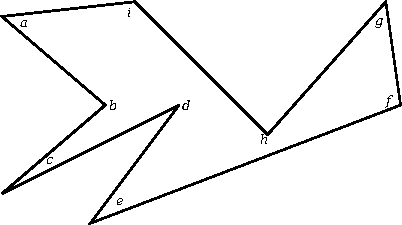
\includegraphics[scale=1.6]{funkyshape.pdf}
\end{image}
Use this table to record your findings:
\[
{\renewcommand{\arraystretch}{1.5}
\begin{array}{|c|c|c|c|c|c|c|c|c|}\hline
a & b & c & d & e & f & g & h & i \\\hline
\rule[7mm]{10mm}{0mm}  & \rule[7mm]{10mm}{0mm}    & \rule[7mm]{10mm}{0mm}   & \rule[7mm]{10mm}{0mm}   &  \rule[7mm]{10mm}{0mm}   & \rule[7mm]{10mm}{0mm}    & \rule[7mm]{10mm}{0mm}   & \rule[7mm]{10mm}{0mm}   & \rule[7mm]{10mm}{0mm}   \\ \hline
\end{array}}
\]
\end{problem}

\begin{problem}
Find the sum of the interior angles of the polygon above. 
\vfill
\end{problem}

\newpage
\begin{problem}
What should the sum be? Explain your reasoning.  
(You might find it useful to consider some of the angles to be ``reflex angles.''  Which ones?)  
\vspace{3in}
\end{problem}


\end{document}
